\documentclass[11pt, A4paper, english]{article}
\usepackage{amsfonts}
\usepackage{amsmath}
\usepackage{amssymb}
\usepackage{amsthm}
\usepackage{babel}
\usepackage{color}
\usepackage{float}
\usepackage[T1]{fontenc}
\usepackage{graphicx}
\usepackage[colorlinks]{hyperref}
\usepackage[utf8]{inputenc}
\usepackage{listings}
\usepackage{textcomp}
\usepackage[style=ieee]{biblatex}
\usepackage{tabularx}

\addbibresource{bibliography.bib}

\definecolor{dkgreen}{rgb}{0, 0.6, 0}
\definecolor{gray}{rgb}{0.5, 0.5, 0.5}
\definecolor{daynineyellow}{rgb}{1.0, 0.655, 0.102}
\definecolor{url}{rgb}{0.1, 0.1, 0.4}

\lstset{frame=tb,
	language=csh,
	aboveskip=3mm,
	belowskip=3mm,
	showstringspaces=false,
	columns=flexible,
	basicstyle={\small\ttfamily},
	numbers=none,
	numberstyle=\tiny\color{gray},
	keywordstyle=\color{blue},
	commentstyle=\color{daynineyellow},
	stringstyle=\color{dkgreen},
	breaklines=true,
	breakatwhitespace=true,
	tabsize=3
}

\lstset{inputpath="C:/Users/Torstein/Documents/skole/USN/IIA2017/Assignment 2"}
\graphicspath{{C:/Users/Torstein/Documents/USN/IIA2017/Assignment 2/}}
\hypersetup{colorlinks, urlcolor=url}

\author{Torstein Solheim Ølberg | 263054}
\title{Assignment 2 in IIA2017}



%\lstinputlisting{Filnavn! type kodefil}. Use [linerange=0-73] or [linerange=73-] to crop
%\includegraphics[width=12.6cm, height=8cm]{Filnavn! type png}



\begin{document}
\maketitle
\clearpage

\tableofcontents
\clearpage

	\section{Introduction}
The industrial automatisation profession is often times occupied with installing and configuring different devices which communicate with each other over a network. Examples of such can be single robots controlled by a computer or whole production lines controlled by set of computers and servers. By studying a computer, its network and communication capabilities, it is possible to learn a lot about how this is done and how best to do it. This report will study a Komplett Khameleon laptop bought in 2020 in Norway.

	\section{Results}
		\subsection{System Information}
From figure \ref{im:ssd_info} we can see that this computer has two storage drives.
			\begin{figure}
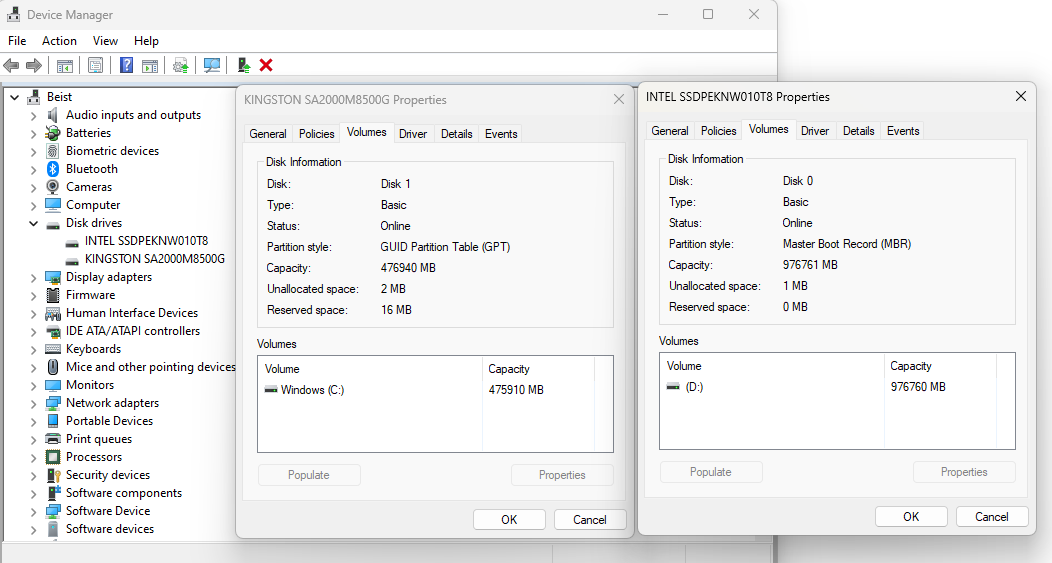
\includegraphics[width=12.6cm, height=8cm]{SSD_info.png}
\caption{Screenshot containing info on the two SSD drives of this computer. The C: drive has about 500 GB of storage space and the D: drive double that amount.}
\label{im:ssd_info}	
			\end{figure}
The first one, C:, has a capacity of approximately 475 GB. From NotebookChecks benchmarking of drive, we know that the interface it uses is NVMe, which is a very fast protocol \cite{Kingston}. As for the D: drive, we see that it has a capacity of approximately 977 GB and from Mouser Electronics, we know that it uses a PCIe interface \cite{Intel}. This also is a very fast interface, but is most often beaten by NVMe if NVMe is combined with PCIe. \\
The number of serial ports is not possible to see on this computer as there is a known error when trying to display this after updating to Windows 10. However, if I normally where to do this, I would have checked the Ports (COM \& LPT) list, but as you can see in figure \ref{im:com_info} there is something wrong with this list. \\ 
The Bluetooth communications devices are listed in figure \ref{im:com_info}
			\begin{figure}
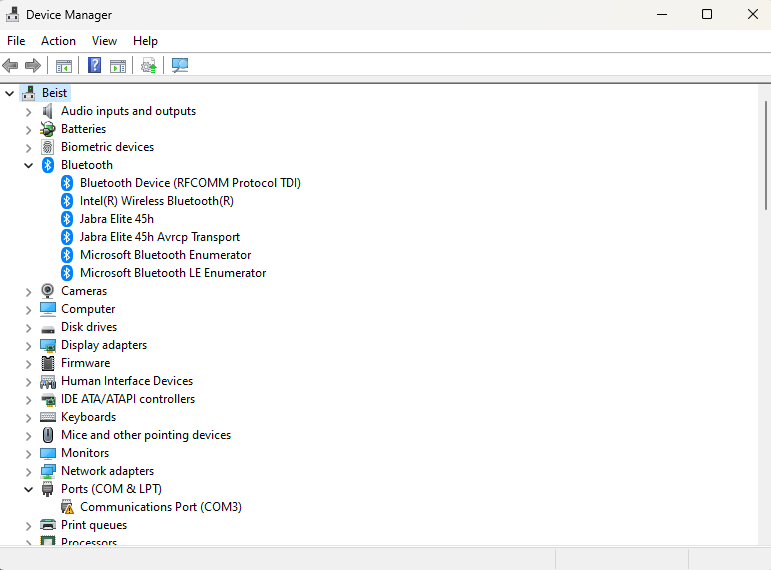
\includegraphics[width=12.6cm, height=8cm]{com_info}
\caption{Screenshot containing info on the available Bluetooth devices for this computer. You can also see there is a fault with the Serial ports list.}
\label{im:com_info}	
			\end{figure}

		\subsection{Communication Directions}
There are three types of protocols for communication directions. First, there is simplex, where communication only goes in one direction. For this, you only need one communication channel. Then there is half-duplex, where communication can go both ways, but only one at a time. This protocol also only needs one channel. Finally, there is duplex, where communication can go both ways at the same time. This protocol needs two channels.

		\subsection{Network Protocols}
The number of network devices can be seen in \ref{im:net_info}.
			\begin{figure}
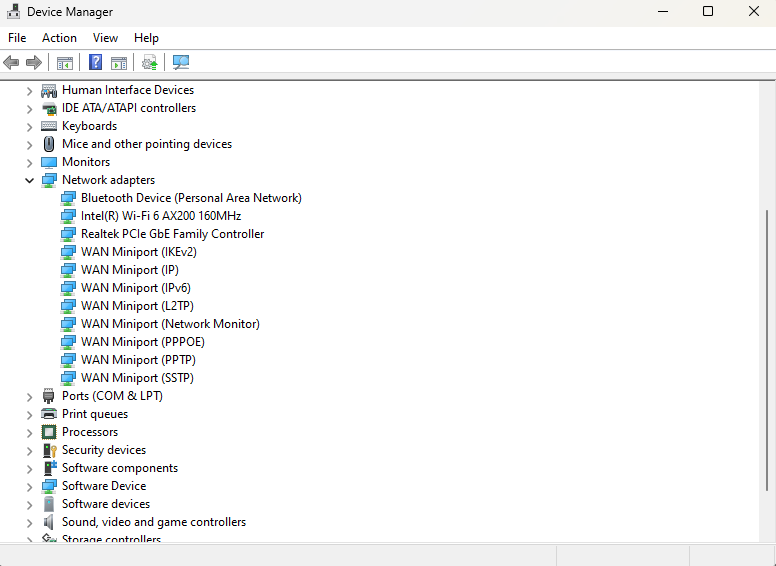
\includegraphics[width=12.6cm, height=8cm]{network_info.png}
\caption{Screenshot containing info on the number and type of each network device on this computer.}
\label{im:net_info}	
			\end{figure}
Here we can see there are eleven network devices. \\
The physical address of my active network is DC-FB-48-01-23-BD as seen in figure \ref{im:net_ad} \\
			\begin{figure}
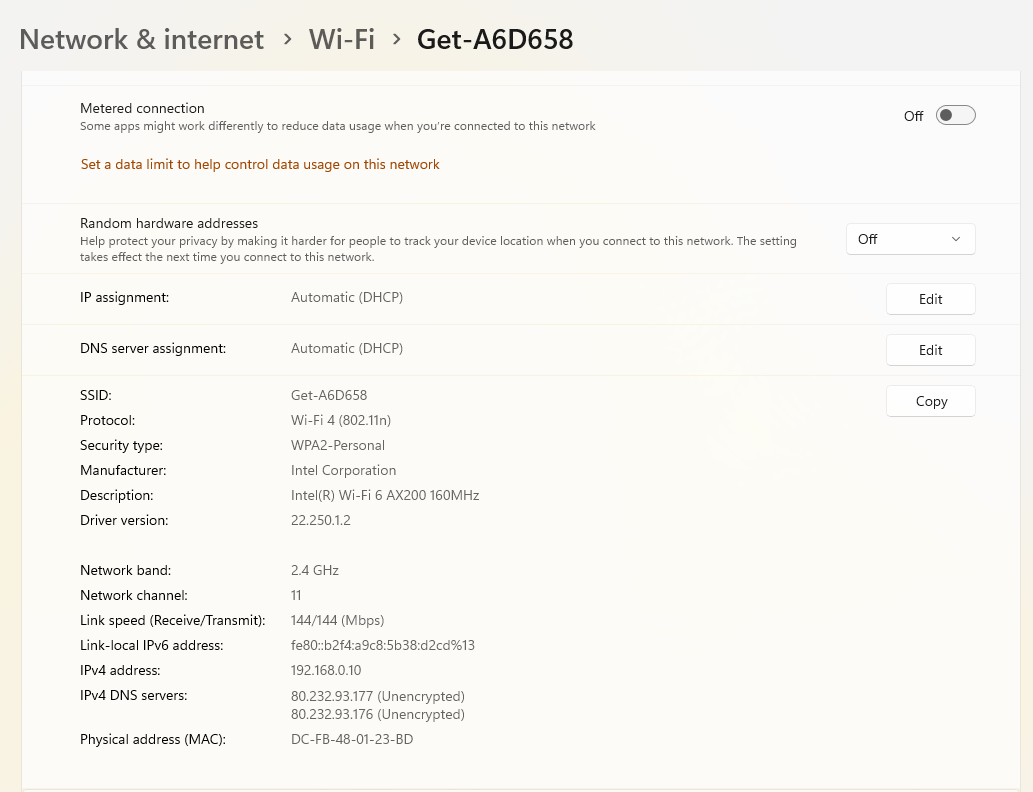
\includegraphics[width=12.6cm, height=8cm]{network_address.png}
\caption{Screenshot containing info on the current active network of this computer. This is a wireless network named Get-A6D658, with a physical and logical address displayed.}
\label{im:net_ad}	
			\end{figure}
The logical address is 192.168.0.10, also seen in figure \ref{im:net_ad} \\
As the logical address starts with 192, we know that it is a class C IPv4 network with a subnet mask of 255.255.255.0 \cite{IPClasses}. Since this address is assigned by a router and no specific adjustment has been done by the user, it is very likely to be a dynamically assigned address. \\
From figure \ref{im:pro_installed}, where netstat -s has ben run to list stats of available network protocols, the it is possible to see that the computer has both TCP and UDP installed.
			\begin{figure}
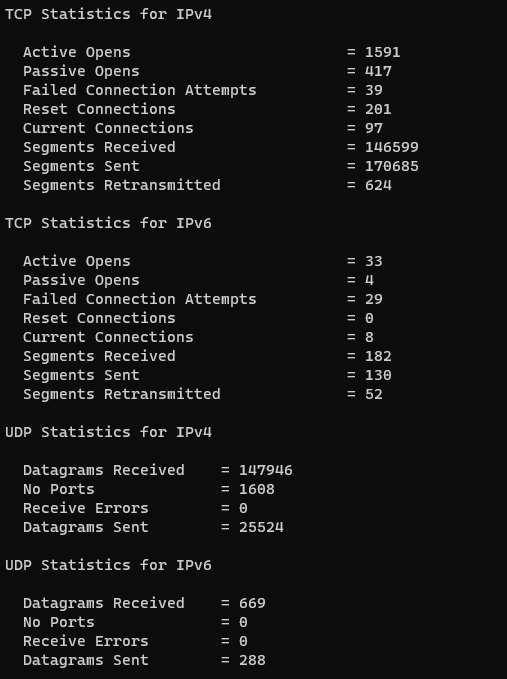
\includegraphics[width=12.6cm, height=12cm]{installed_protocols.png}
\caption{Screenshot containing info on which protocols have been installed on this computer. We see that TCP IPv4 and IPv6 as well as UDP IPv4 and IPv6. has been installed.}
\label{im:pro_installed}	
			\end{figure}
It is also possible to see that the computer supports both TCP IPv4 and IPv6. \\

			\subsubsection{Wireless}
If I had to choose between the three networks listed in figure 2.1 in \cite{Assignment}. I would choose the top one as it has a greater signal strength. \\
The authentication to this network is unknown, so likely it needs some sort of password to access. \\
The reason we do not see any other networks than the LAN is because wo connect to a WAN via the LAN. \\
The first network is a direct connection to another device. It is likely privately owned, possibly by someone named Thamm, and has no security. It also seems to be quite far away, or disrupted by a lot of walls, as it has a very faint signal strength. The other networks all have some sort of access security and are general networks. CM is the closest one, with strong signal, The other four are all quite faint, and likely controlled by the same owner which likes science fiction. \\
As for the networks available at the location of this computer, they can be seen in figure \ref{im:av_net}. 
				\begin{figure}
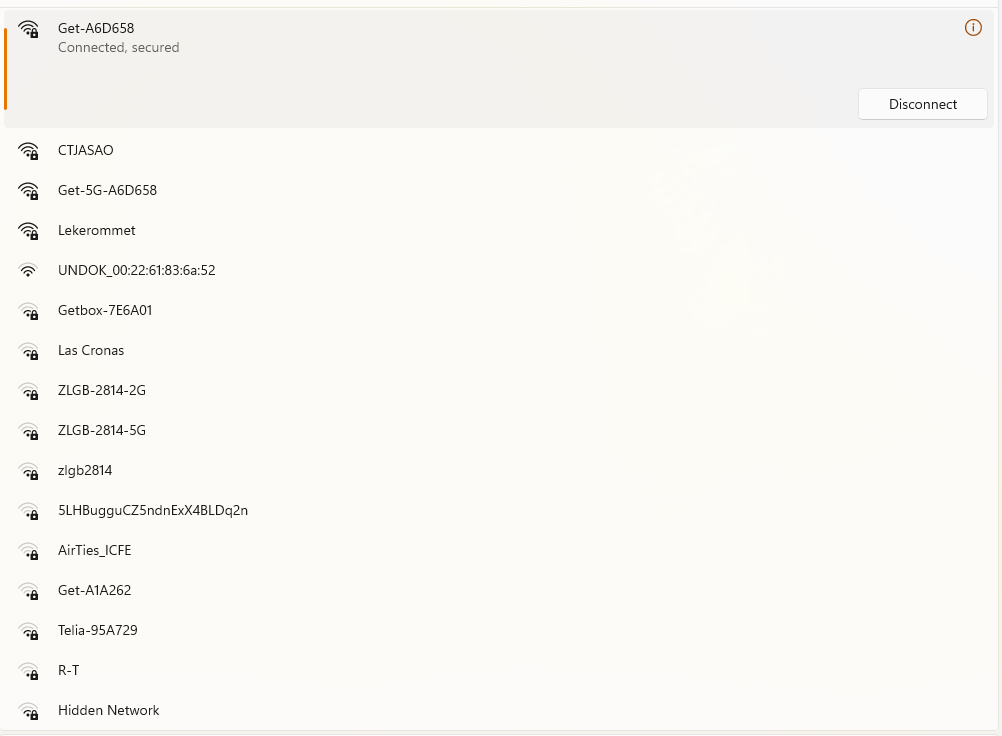
\includegraphics[width=12.6cm, height=8cm]{available_networks.png}
\caption{Screenshot containing info on the available networks in this computers location.}
\label{im:av_net}	
				\end{figure}

			\subsection{Network Test}
Starting with pinging \url{tv.nrk.no}. In figure \ref{im:ping_nrk} we can see an attempt at pinging this website four times and all of them where successful.
				\begin{figure}
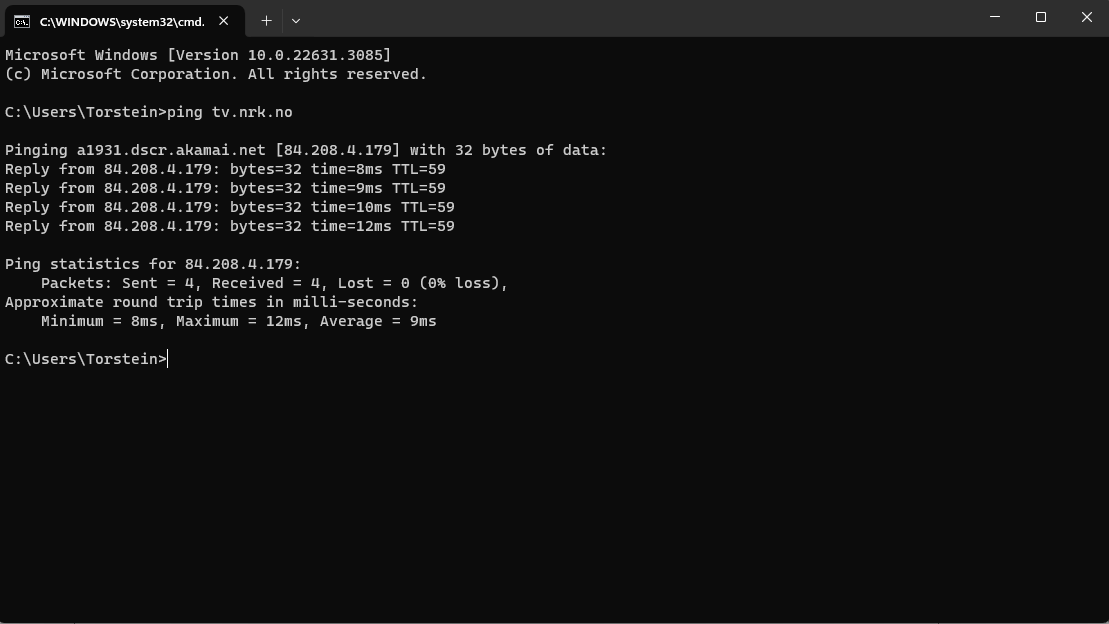
\includegraphics[width=12.6cm, height=8cm]{ping_nrk.png}
\caption{Screenshot of a ping of tv.nrk.no. The ping was done four times, all of them successful, and generally quite quick.}
\label{im:ping_nrk}	
				\end{figure}
The ping was generally quick, with a minimum time of 8ms and a max time of 12ms. If we try to ping it continuously, and trace the messages with WireShark, we can see from figure \ref{im:con_ping_nrk} that IPv4 is used and that the logical address of the website is 84.208.4.179.
				\begin{figure}
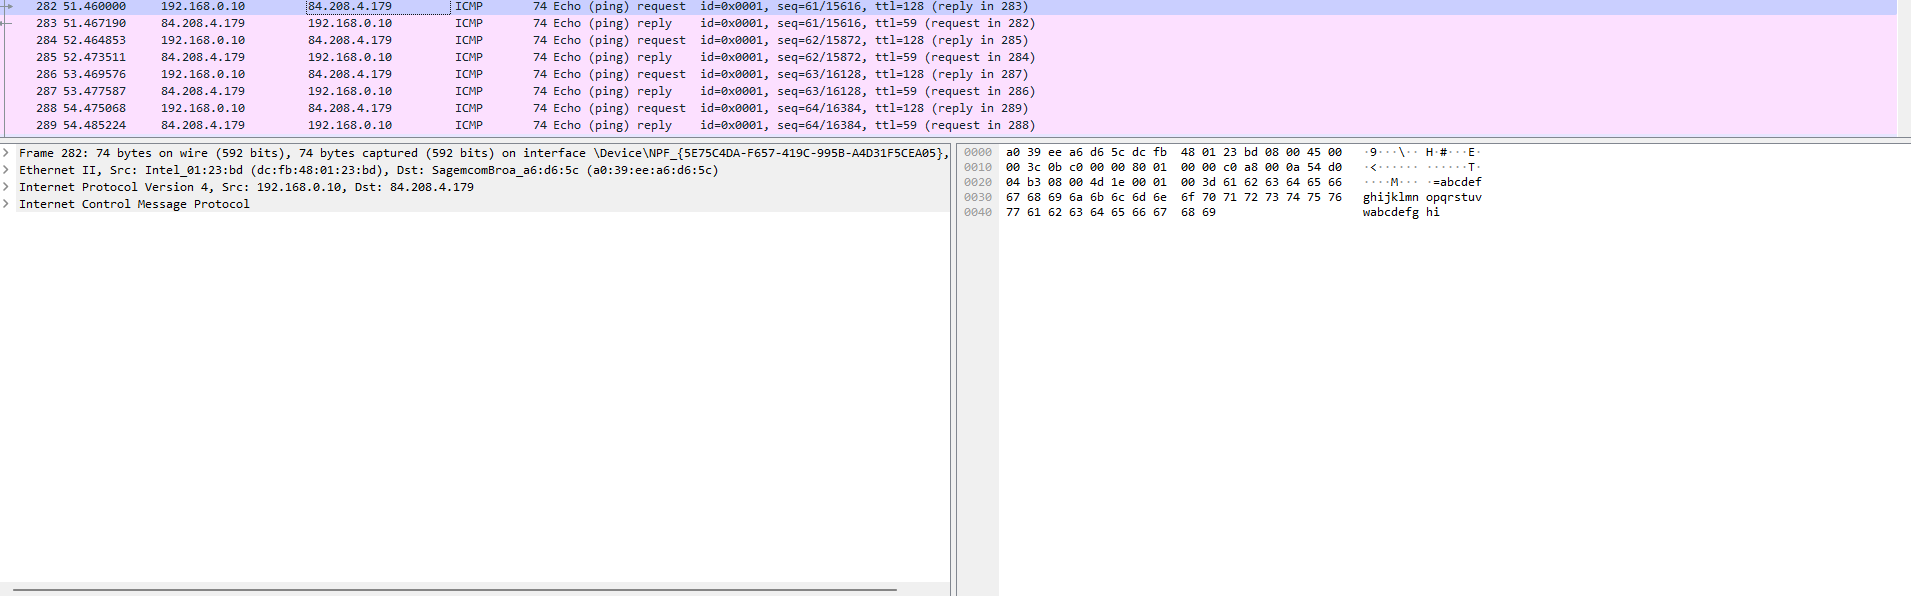
\includegraphics[width=12.6cm, height=8cm]{continous_ping_nrk.png}
\caption{Screenshot of WireShark displaying info on a ping request of the website tv.nrk.no. We can see the logical address of both the requester and the website}
\label{im:con_ping_nrk}	
				\end{figure}
A ping application can easily be made in C\# to help perform pings and to control what data is sent. One such application has been created by Nils-Olav Skeie and can be seen in the appendix \cite{Assignment}. Changing the data and host of the original application to tv.nrk.no and the string CanIWatchPoirot? we can run the application and see that we get a response. A run of this application can be seen in figure \ref{im:app_test} where we see that the website has been pinged, it has the same address as earlier, and managed a round trip in 6ms.
				\begin{figure}
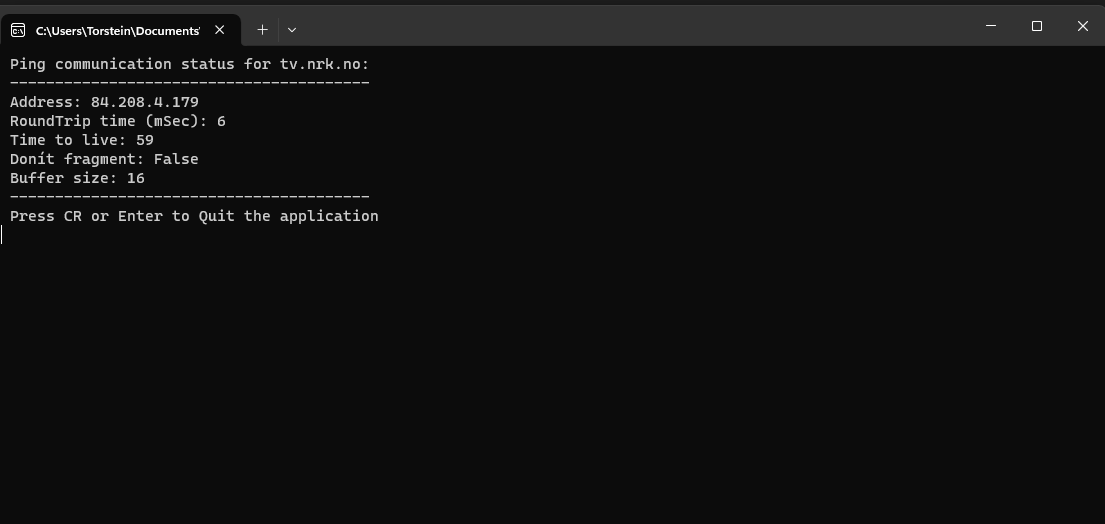
\includegraphics[width=12.6cm, height=8cm]{app_test.png}
\caption{Screenshot of a run of the PingApp application. The name, address and trip time has been displayed.}
\label{im:app_test}	
				\end{figure}
A known problem with the communication performed in circumstances as we have just done are that the protection of the information transmitted with TCP/IP is not that good. Another application can easily gain access to the info transmitted, as seen in figure \ref{im:app_test_WS}.
				\begin{figure}
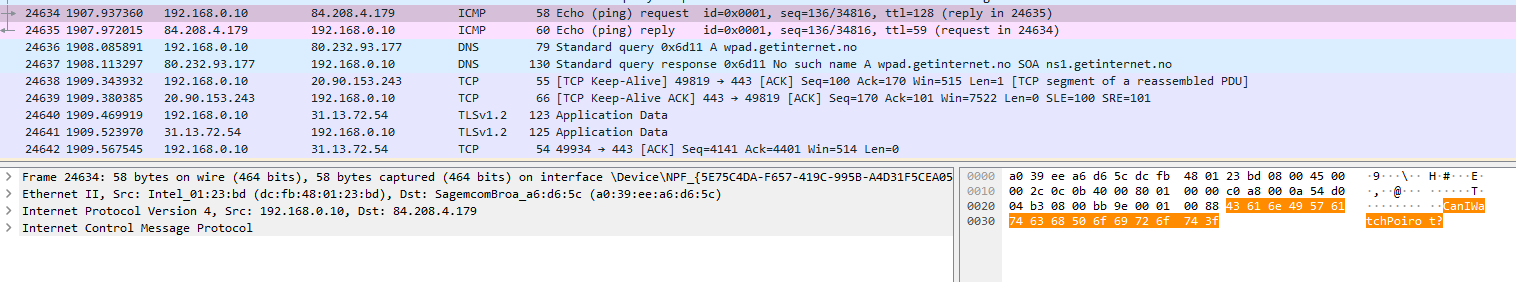
\includegraphics[width=12.6cm, height=5cm]{plaintext.png}
\caption{Screenshot of run of the application PingApp traced in WireShark. We can see the data sendt in plaintext.}
\label{im:app_test_WS}
				\end{figure}
The data packages are sent in plain text and anyone whom intercepts the data can read it. \\
The application could be extended by adding a way to ping multiple times in a row and perform an averaging of the results. This could be done by adding something like this code to the program.
				\begin{lstlisting}
def average_pinger(int nr_pings):
{
	string data = "message"
	string host = "website.com"
	float total_time = 0
	for i from 0 to nr_pings:
	{
		reply = Ping(host, Encrypt(data))
		total_time += reply.RounttripTime
	}
	WriteToConsole("The average time for a ping was " + total_time / nr_pings + "seconds")
}
				\end{lstlisting}
A tool for pinging all the nodes in a network segment is also usefull. This could be implemented by code like the on showed underneath.
				\begin{lstlisting}
def ping_segment(string network_prefix):
{
	string data = "message"
	for i from 0 to 255:
	{
		string host = network_prefix + i
		reply = Ping(host, Encrypt(data))
		WriteToConsole("Pinged " + host + ": Status = " + reply.status)
	}
}
				\end{lstlisting}
This code loops through all possible addresses for nodes on the network segment and pings all. Then it displayes if the ping was answered or not. An implementation of this code in the PingAppcan be seen in the appendix.

		\subsection{Digitalization}
When choosing to digitilaze a system, it could be better to choose a plain text format rather than a database. An application taking sensor values an logging them to a text file would be useful. One such application was created by Torstein Solheim Ølberg \cite{DAQ}. A version of this application, using different samplingtime and semicolon as separator instead of comma, can be viewed in the appendix. \\
A flowchart, documenting the buildup of the application can be seen in figure \ref{im:flowchart}. \\
This application could, be further developed by adding a low-pass filter between the sensors and the logging, such that any noise or problematic data points could be removed. This would be implemented by allowing the sensors to return values outside the expected range and checking the values before saving them to the sample list. Another possible addision would be to add support for other types of files to save to. The csv file is a text file where data is recorded in plain text, separated by commas, or in our case semicolons as seen in figure \ref{im:csv}.
			\begin{figure}
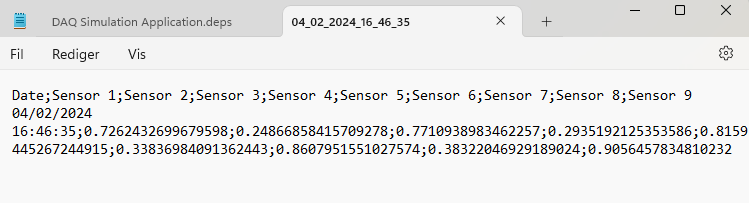
\includegraphics[width=12.6cm, height=3cm]{csv.png}
\caption{Screenshot of data stored by the DAQ simulation application.}
\label{im:csv}
			\end{figure}
This makes it a simple file to record to, but it is not very flexible. Another type of data storage file is XML. In this file format, data is stored within tags, making for a much more customizable way of categorising the data stored. This format also allows for data to be stored in a way that is readalbe for people, but since there are tags, it is much more easy for computers to extract the info in a useful way. A third option is the jfon file. Json is also a format readable by humans, but instead of using tags like XML, it uses objects. Data stored in objects are easy to group togeter, but adding information to it can be more difficult. It is the grouping ability of Json which makes it a very good pick for this applications choice. All of these file formats are however not optimal when it comes to security. This is because all of them store data in a human readable format. For the use of simulating any random sensor, it is not important to protect the data as the risk is not very high for the data to be misused. However, if the data sored is important it would be smart to use a file format where the data is encryped. If the fileformat encryped in a standard way, a real percistant threat could however decrypt it using a program, so if the data is really important, decypion using a key only authorised people know would be a smart choice.

		\subsection{Cloud Systems}
IAAS or Infrastructure As A Service is a cloud service model where servers, networks and infrastructure is offerend on-demand to customers, where they can create their own applications without needing to wory about physical space or maintenance crew. SAAS, or Software As A Service however is cloudbased access to fully operational software for applications. \\
The DAQ Simulation Application can be extended to also work with a cloud based system. As to not force the sensors to be physically pluged into the computer runing such an application, it is possible to transfer the data to the application through the use of an API, an Application Programming Interface. If this cloud system sends the data to the application, it would also be useful to store the data, once processed by the application, into a cloud stored file. This can be done in multiple ways, for example by using a different application which continously backs up files stored on the computer, or by using the DAQ Application to save the file to an online server. Here it would be simple to use SAAS like Google Drive Dropbox, which allows for directly saving files to their online servers.


	\section{Conclusion}
		\subsection{This Computer}
From this analysis, this computer has a wide set of very quick communication methods, both internaly and over internet. There are multiple network protocols installed, it is possible to display tis information as well as use it to communicate.
		
		\subsection{Network testing}
The active network this commputer is on is a LAN, connected to the internet via TCP IPv4, where a ping attempt to a webgsite uses a short roundabout time. It is also possible to create a simple application which can be used to ping different nodes. This does however display a security risk in that information sendt via the protocl used is sendt in plain text and can thus be intercepted and read by anyone.
		
		\subsection{DAQ Application}
A simple Data aquisition application can be created and used to aquire data from different sensors and store them to a csv file or other format. This application could also be extended to include the possibility of reading from and writing to a cloud based service.

\noindent \begin{tabularx}{\linewidth}{@{}X|X|X|X|X}
Sections 						& Weighting (\%)	& Your evaluation (\%) 	& Review (\%) 	& Comments \\
\hline
System Information 				& 2.5				& 15					&  				& Finding out the problem with Ports took a lot of work. \\
\hline
Network Information 			& 20				& 35 					&  				&  \\
\hline
Network Testing					& 35				& 25 					&  				&  \\
\hline
Digitalization	 				& 30				& 10					&  				& I reused a lot of code from a different project. \\
\hline
Cloud Systems 					& 10				& 12.5					&  				&  \\
\hline
Conclusion		 				& 2.5				& 2.5					&  				&  \\
\hline
Sum					 			& 100				&  						&  				& 
		\end{tabularx}

\printbibliography
	
	\section{Appendix A}
Here you can find the documentation for the program. \\
		\begin{figure}[H]
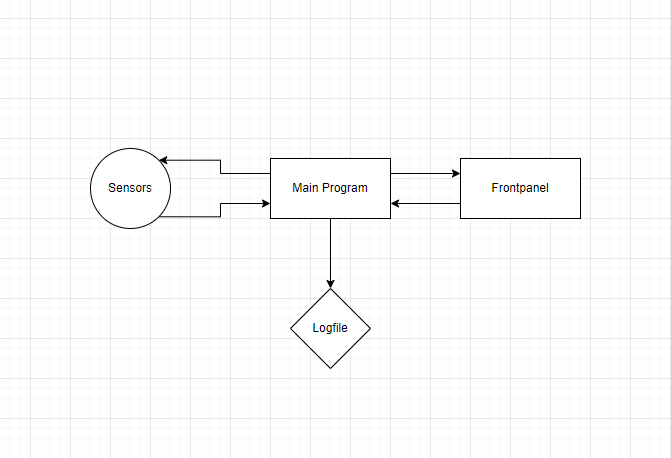
\includegraphics[width=12.6cm, height=8cm]{Flowchart.png}
\caption{Flowchart documentation of the DAQ simulation application.}
\label{im:flowchart}
		\end{figure}

	\section{Appendix B}
Here you can find the code files not made by Visual Studio itself.
\lstinputlisting[linerange=0-73]{PingApp/Program.cs}
\lstinputlisting[linerange=73-]{PingApp/Program.cs}
\lstinputlisting{DAQ Simulation Application/SensorApp.cs}

\end{document}